\documentclass[10pt]{article}
\usepackage{/home/liam/4thlabs/latex/lab}


\title{Assignment 1 - Advanced Computational Science}

\newcommand{\ujn}{u_{j}^{n}}
\newcommand{\ujpn}{u_{j+1}^{n}}
\newcommand{\ujmn}{u_{j-1}^{n}}
\newcommand{\ujnp}{u_{j}^{n+1}}
\newcommand{\ujnm}{u_{j}^{n-1}}
\newcommand{\eihjk}{e^{ikhj}}
\newcommand{\eihjpk}{e^{ikh(j+1)}}
\newcommand{\eihjmk}{e^{ikh(j-1)}}

\begin{document}
\maketitle

\section*{Question 1}
\subsection*{(1)}
We are interested in solving the 1-d wave equation with $c=1$,
\begin{equation}
\frac{\partial^2 u}{\partial t^2} = \frac{\partial^2 u}{\partial x^2}
\label{e:we}
\end{equation}
using central differences,
\begin{equation}
\frac{\partial^2 u}{\partial t^2} \approx \frac{\delta_t^2 \ujn}{\tau^2},
\hspace{5mm}
\frac{\partial^2 u}{\partial x^2} \approx \frac{\delta_x^2 \ujn}{h^2}
\label{e:central}
\end{equation}
so our equation becomes
\begin{equation}
\frac{\delta_t^2 \ujn}{\tau^2} = \frac{\delta_x^2 \ujn}{h^2}
\label{e:wecd}
\end{equation}
where $\tau$ is the time step size, and $h$ is the $x$ step size.

The operator $\delta_x ^2$, when applied to $\ujn$, gives
$$
\delta_x^2 = \ujnm - 2\ujn + \ujnp
$$
allowing us to expand out for both spatial and temporal derivatives and rearrange
for $\ujnp$, giving
\begin{equation}
\ujnp = \nu^2 \left[\ujmn + \ujpn \right] - \ujnm + 2(1 - \nu^2)\ujn
\label{e:cd}
\end{equation}
with $\nu = \frac{\tau}{h}$.

A program was written in Python 3.3 to solve this problem with Dirichlet boundary
conditions, $u(-7,t) = u(7,t) = 0$, on the intervals $x \in \left[-7,7\right]$,
$t \in \left[0,14\right] $. The initial condition is given by
$u(x,0) = e^{-x^2}$.
The program is included in appendix \ref{a:1.1}.

The solutions at various times are shown in figure \ref{f:dirichlet}.
\begin{figure}
  \centering
  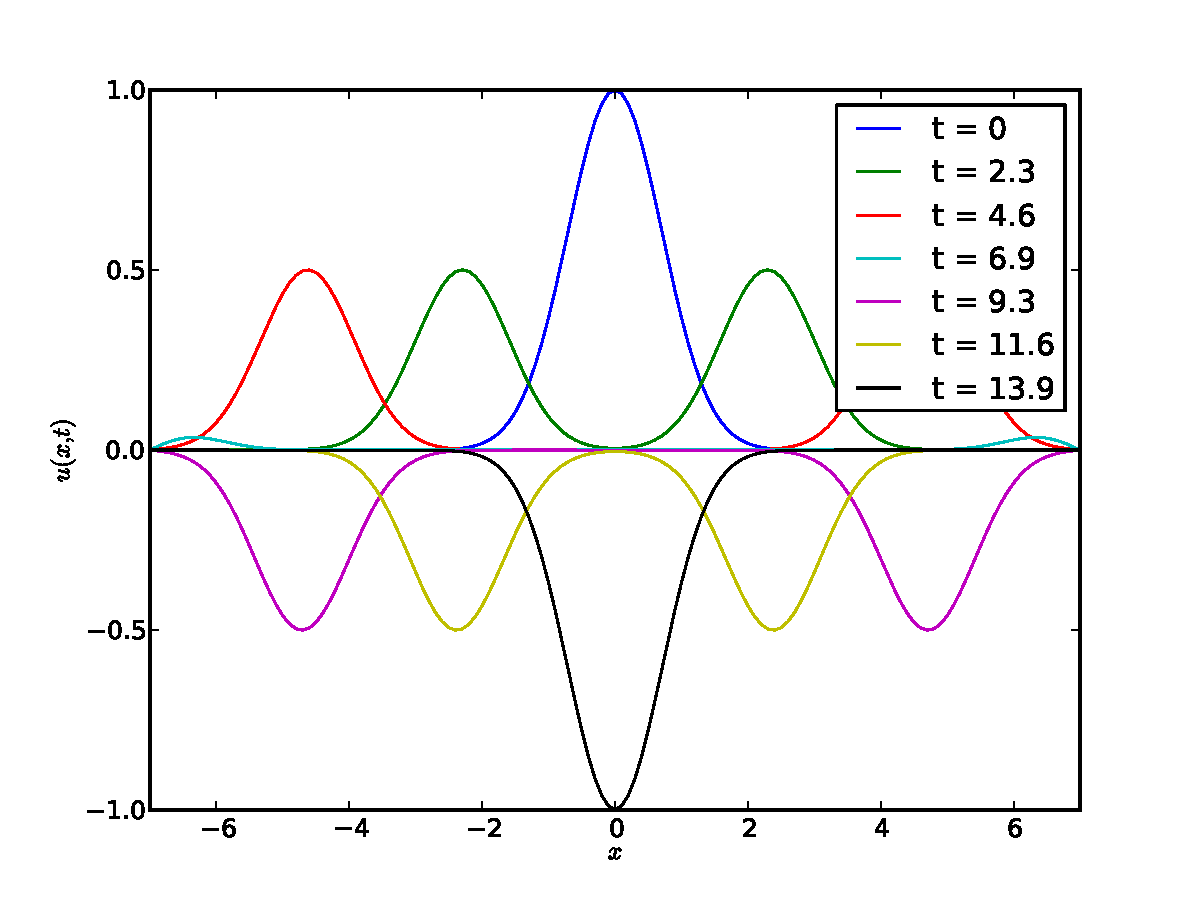
\includegraphics[width=\textwidth]{1/dirichlet.pdf}
  \caption{Solution to the wave equation with Gaussian initial condition.}
  \label{f:dirichlet}
\end{figure}

\subsection*{(2)}
Our expression for $\ujn$ using Central Differences is given in equation \ref{e:cd}.
To perform Fourier/von Neumann stability analysis, we take $\ujn = \xi^n \eihjk$ as
a single Fourier mode solution, and see how our {\it amplification factor}, $\xi$,
behaves as a function of $\tau,h,k$.
Substituting this into equation \ref{e:cd} gives
$$
\xi^{n+1} \eihjk= \nu^2 \left[ \xi^n \eihjmk + \xi^n \eihjpk \right] - \xi^{n-1} \eihjk +
2(1 - \nu^2) \xi^n \eihjk.
$$
Dividing across by $\xi^{n-1} \eihjk$ and cleaning up gives
$$
\xi^2 + \alpha \xi + 1 = 0
$$
with
$$\alpha = -\nu^2 \left[ e^{-ikh} + e^{ikh} - 2\left(1 - \frac{1}{\nu^2}\right) \right]
= -2 \nu^2 \left[ \cos(kh) - \left(1 - \frac{1}{\nu^2}\right) \right] $$
$$= -2 \nu^2 \left[ 1 - \sin^2\left(\frac{kh}{2}\right) - \left(1 - \frac{1}{\nu^2}\right) \right]
=  2 \nu^2 \left[ \sin^2\left(\frac{kh}{2}\right) - \frac{1}{\nu^2} \right] $$
This is a quadratic equation with roots
$$
\xi_\pm = \frac{1}{2} \left( -\alpha \pm \sqrt{\alpha^2 - 4} \right) =
\frac{1}{2} \left( -\alpha \pm i\sqrt{(2 - \alpha)(2+\alpha)}\right).
$$
Inserting $\alpha$ into the above gives
$$ \xi_\pm = -\frac{1}{2}\left[2\nu^2 \sin^2\left(\frac{kh}{2}\right) -1 \right]
\pm \frac{1}{2}\sqrt{\left(4\nu^2\sin^2\left(\frac{kh}{2}\right) -2\right)^2 - 4}
$$
$$ = -\left[2\nu^2 \sin^2\left(\frac{kh}{2}\right) -1 \right]
\pm \nu\sin\left(\frac{kh}{2}\right)\sqrt{4\nu^2\sin^2\left(\frac{kh}{2}\right) -2}
$$

From here, it is immediately apparent that if $\nu >1$, both terms will be greater
than $0$ for some values of $k$, making the method unstable.

\subsection*{(3)}
The program used is included in appendix \ref{a:1.3}.


\section*{Question 2}
\subsection*{(1)}
We are now asked to solve the wave equation with $c=1$ and external potential
$V(x) = \frac{1}{\cosh^2(x)}$.
I chose to use central differences -- equation \ref{e:central} -- once again as it
is simple to program and showed no significant shortcomings in the previous
section which cannot be fixed by computational power.
By the same method as for question 1.1, we can use central differences for this
equation. This gives
\begin{equation}
\ujnp = \nu^2 \left[\ujmn + \ujpn \right] - \ujnm + 2(1 - \nu^2)\ujn - \tau^2 V_j \ujn
\label{e:cdp}
\end{equation}
where $V_j$ is the potential corresponding to the $x$-value $j$. The effect of
$V$ can be seen to scale with the time step $\tau$, which is intuitive.

The program was written in Python 3 again, and is in appendix \ref{a:2.1}.
A plot of the waves behaviour is shown in figure \ref{f:cosh}.
The wave interacts with the barier, and some is transmitted, while more
is reflected.

\begin{figure}
  \centering
  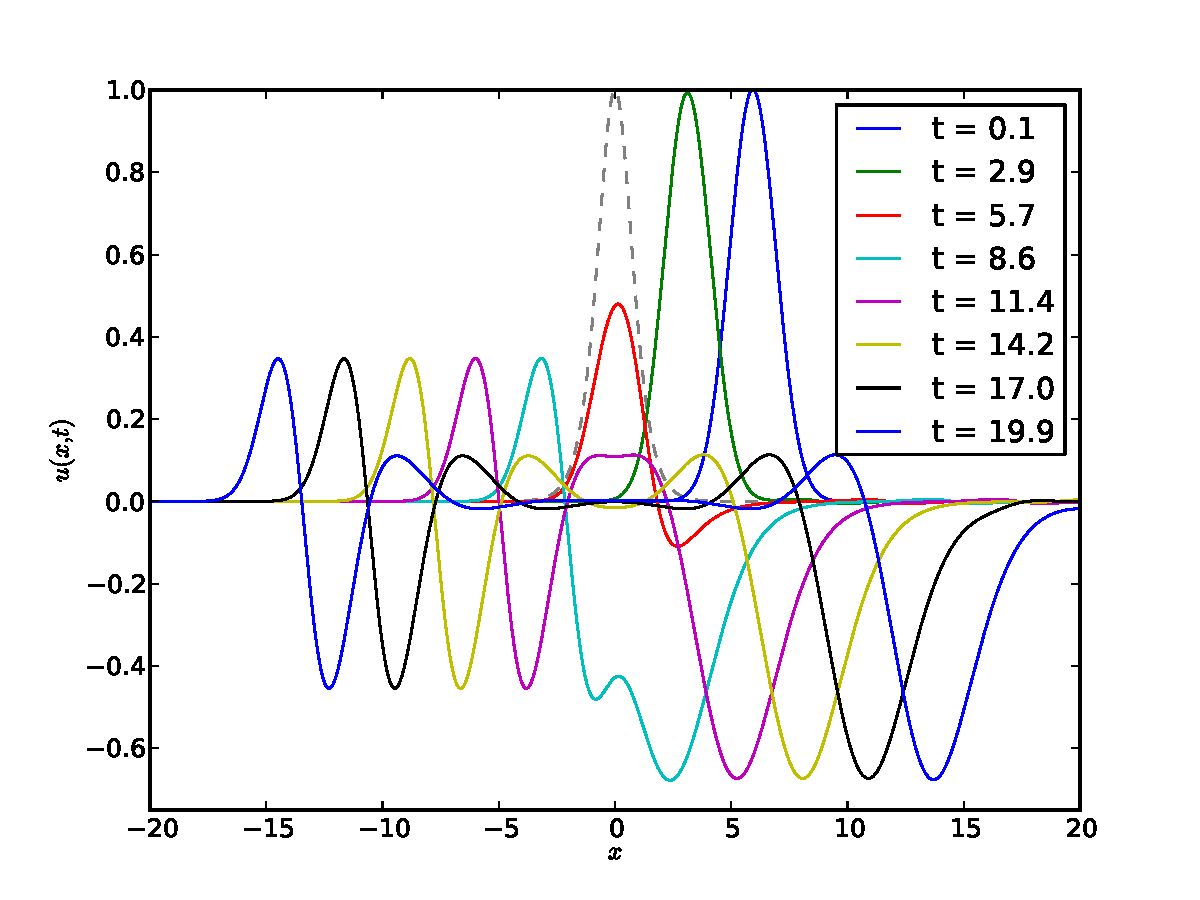
\includegraphics[width=\textwidth]{2/cosh.pdf}
  \caption{The wave at various times, with the potential plotted in the dashed red line.}
  \label{f:cosh}
\end{figure}



\subsection*{(2)}


\subsection*{(3)}


\subsection*{(4)}


\newpage
\begin{appendix}
\section{Program for 1.1}
\label{a:1.1}
\lstinputlisting[language=python]{1/dirichlet.py}
\newpage
\section{Program for 1.3}
\label{a:1.3}
\lstinputlisting[language=python]{1/hstudy.py}
\newpage
\section{Program for 2.1}
\label{a:2.1}
\lstinputlisting[language=python]{2/potential.py}
\newpage
\section{Program for 2.2}
\label{a:2.2}
\lstinputlisting[language=python]{2/hstudy.py}
\end{appendix}



\end{document}
